

\section{Final Results \label{sec:results}}
In this section we discuss the results of the statistical
interpretation of the \scalht dependent yield measurements 
in the all-hadronic, W+jet, and Photon+Jet samples. 
%We consider two interpretation scenarios:
%\begin{itemize}
%\item[a)] zero QCD contamination throughout the entire HT region-of-interest; and constant \RaT as a function of \scalht for the remaining EWK backgrounds (as described in section 2.2)
%\item[b)]  small QCD contamination in the lower \scalht bins described by a single exponential function (see section 4.2.1); and constant \RaT as a function of \scalht for the dominant EWK background     
%\end{itemize}
We consider the following scenario: small QCD contamination mainly in the
lower \scalht bins described by a single exponential function (see
Section 4.2.); and constant \RaT as a function of \scalht for the
dominant EWK background 

The \scalht distributions shown in Figure~\ref{fig:hadronic},
~\ref{fig:muon}, and ~\ref{fig:photon} are the result of the 
simultaneous fit to the \scalht dependent yield in the all-hadronic,
W+jet and photon+jet sample, respectively. 
%For both interpretation scenarios, 
A good agreement 
between the measured \scalht distributions and the best fit is 
observed in all three distributions, indicating that the number of
events found in data is compatible with the SM background expectation 
predicted by the fit.  
%With a p-value of 0.75 for scenario a) and a p-value of  0.82 for
%scenario b), both interpretation hypothesise for the \scalht
%dependences of \RaT  are well reproduced (see Figure~\ref{fig:rat}).  
With a p-value of 0.56, the hypothesis for the \scalht
dependences of \RaT  is well reproduced (see Figure~\ref{fig:rat}).
However, both QCD fit parameters,  $A_{QCD}=(1.4 \pm 1.9) \times
10^{-5}$ and $k_{QCD}=(5.2 \pm 5.6)\times 10^{-3}$, 
are compatible with zero indicating that no significant QCD
contamination has been observed in the signal region. 
%This in turn validates scenario a), which makes the explicit
%assumption of zero QCD contamination. 
%However, for the final result presented here, we have decided to
% chose the more conservative scenario b), which allows for a small 
%potential QCD contamination in the low \scalht part of the signal
%region.
The fit results are tabulated in Table~\ref{tab:results-fit}. 
%A very similar result is obtained from scenario a).

We interpret this lack of signal as a limit on
the allowed parameter space of the CMSSM. In each point of the parameter scape, the SUSY particle spectrum is calculated
using SoftSUSY \cite{Allanach:2001kg}, and the signal events are
generated at leading order (LO) with \PYTHIA6.4~\cite{pythia}.  NLO cross sections, obtained with the program Prospino~\cite{Beenakker:1996ch}, 
are used to calculate the observed and expected exclusion contours. The simulated signal events are re-weighted to match the average number of pile-up events observed in data.



\begin{table}[ht!]
\caption{Fit Results for 1.1fb$^{-1}$. Since the QCD fit parameters are compatible with zero (see text), the listed QCD contributions in this table are also compatible with zero. }
\label{tab:results-fit}
\centering
\footnotesize
\begin{tabular}{ c|c|c|c|c }

\hline
\scalht Bin (GeV)       & 275--325                       & 325--375                       & 375--475                       & 475--575                       \\ [0.5ex]
\hline
W + $\ttNew$ background & 363.7                          & 152.2                          &  88.9                          &  28.8                          \\ 
$\znunu$ background     & 251.4                          & 103.1                          &  86.4                          &  26.6                          \\ 
QCD background          & 172.4                          &  55.1                          &  26.9                          &   5.0                          \\ \hline
Total Background        & 787.4                          & 310.4                          & 202.1                          &  60.4                          \\ 
Data                    & 782                            & 321                            & 196                            & 62                             \\ 

\hline
\scalht Bin (GeV)       & 575--675                       & 675--775                       & 775--875                       & 875--$\infty$                  \\ [0.5ex]
\hline
W + $\ttNew$ background &  10.6                          &   3.1                          &   0.6                          &   0.6                          \\ 
$\znunu$ background     &   8.7                          &   4.3                          &   2.5                          &   2.2                          \\ 
QCD background          &   1.0                          &   0.2                          &   0.1                          &   0.0                          \\ \hline
Total Background        &  20.3                          &   7.7                          &   3.2                          &   2.9                          \\ 
Data                    & 21                             & 6                              & 3                              & 1                              \\ 

\hline
\end{tabular}
\end{table}

Figure~\ref{fig:cmssm} shows the observed and expected 95\% CL exclusion limits in the 
$m_0$-$m_{1/2}$ plane for $\tan \beta = 10$ and $A_0 = 0 \gev$
calculated with a two-sided profile likelihood method. 
Squark and gluino masses of 1.25 \TeV can be
excluded for values of the common scalar mass at the GUT scale  
$m_0 < 530 \gev$. When calculating the observed limit using the \cls method~\cite{cls-pdg}, squark and gluino masses of 1.1 \TeV can be
excluded for $m_0 < 500 \gev$.

% \begin{figure}[t]
%   \begin{center}
%     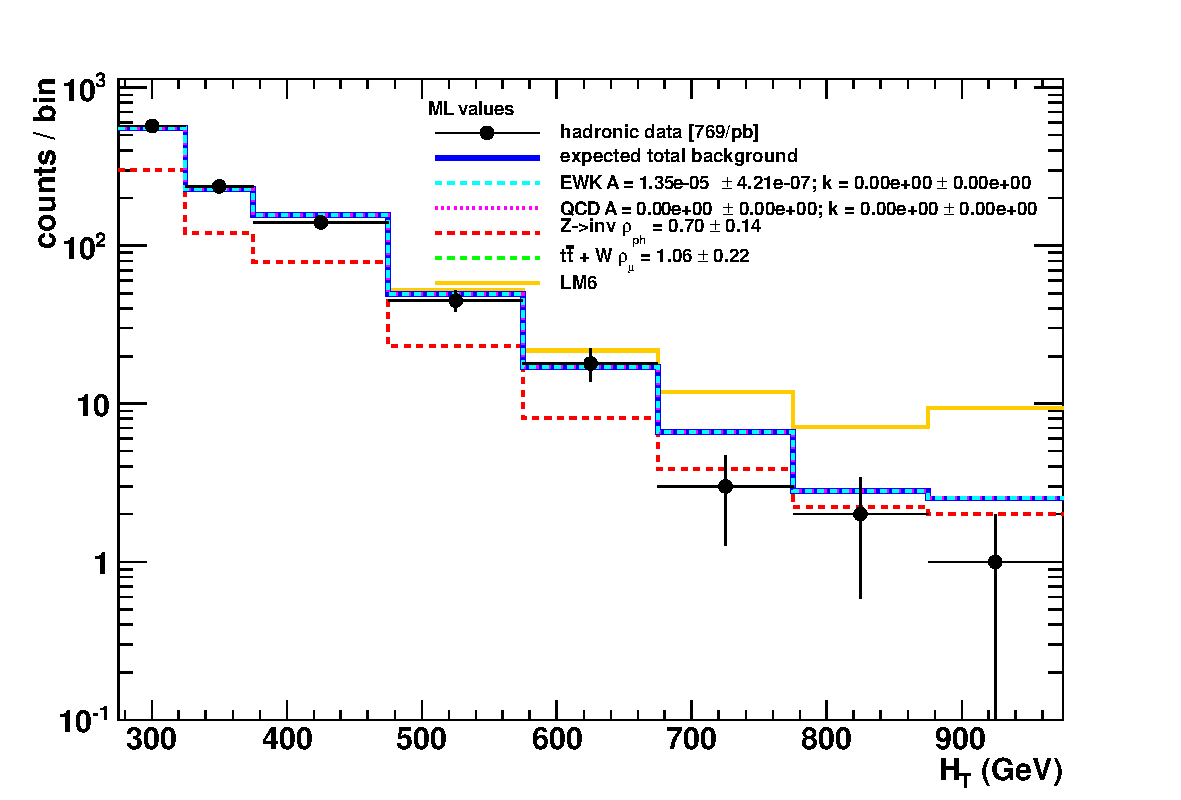
\includegraphics[width = 0.48\textwidth]{figures/stats_plots/RQcdZero/hadronic_signal_fit_logy.pdf}
%     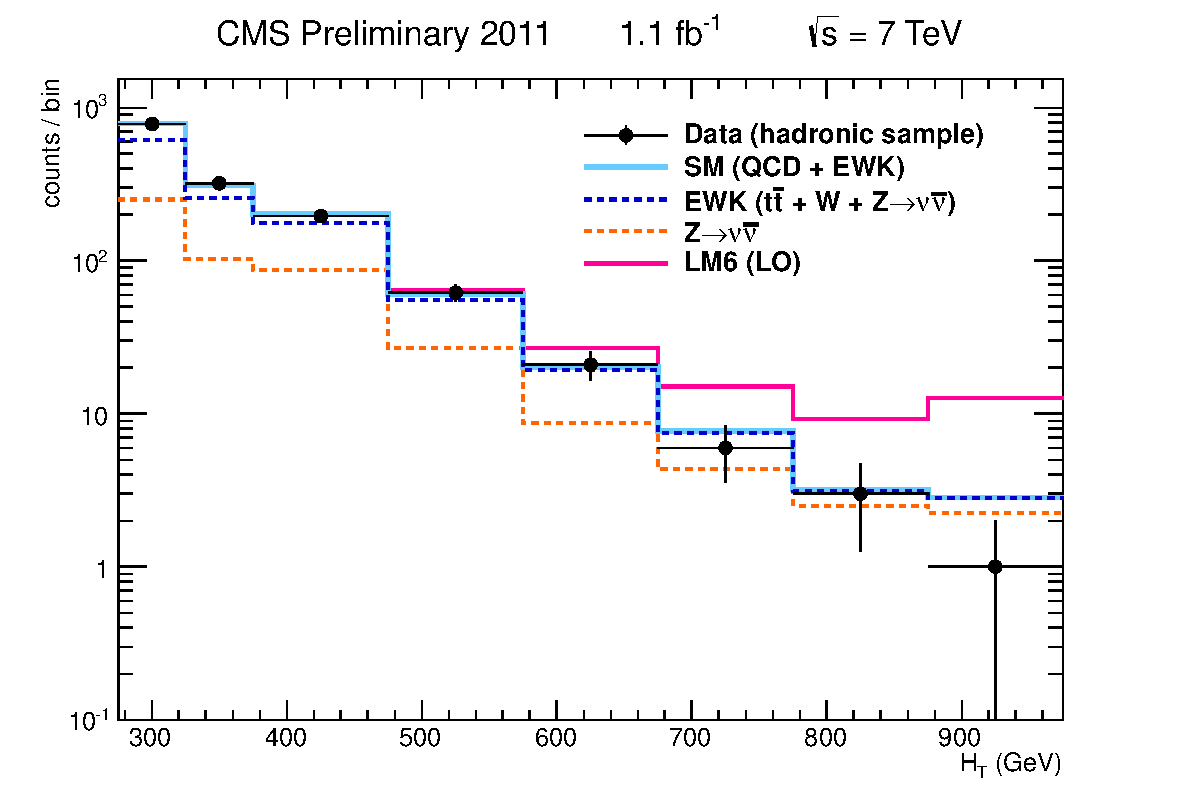
\includegraphics[width = 0.48\textwidth]{figures/stats_plots/RQcdFallingExp/hadronic_signal_fit_logy.pdf}
%     \caption{\label{fig:hadronic} \scalht distribution for events in the hadronic signal sample for scenario a) (left) and scenario b) (right). Shown are the events observed in data (black points), the outcome of the fit (blue line) and a breakdown of the individual background contributions as predicted by the control samples. A possible signal contribution from benchmark point LM6 is indicated as well (yellow line).}
%   \end{center}
% \end{figure}

% \begin{figure}[t]
%   \begin{center}
%     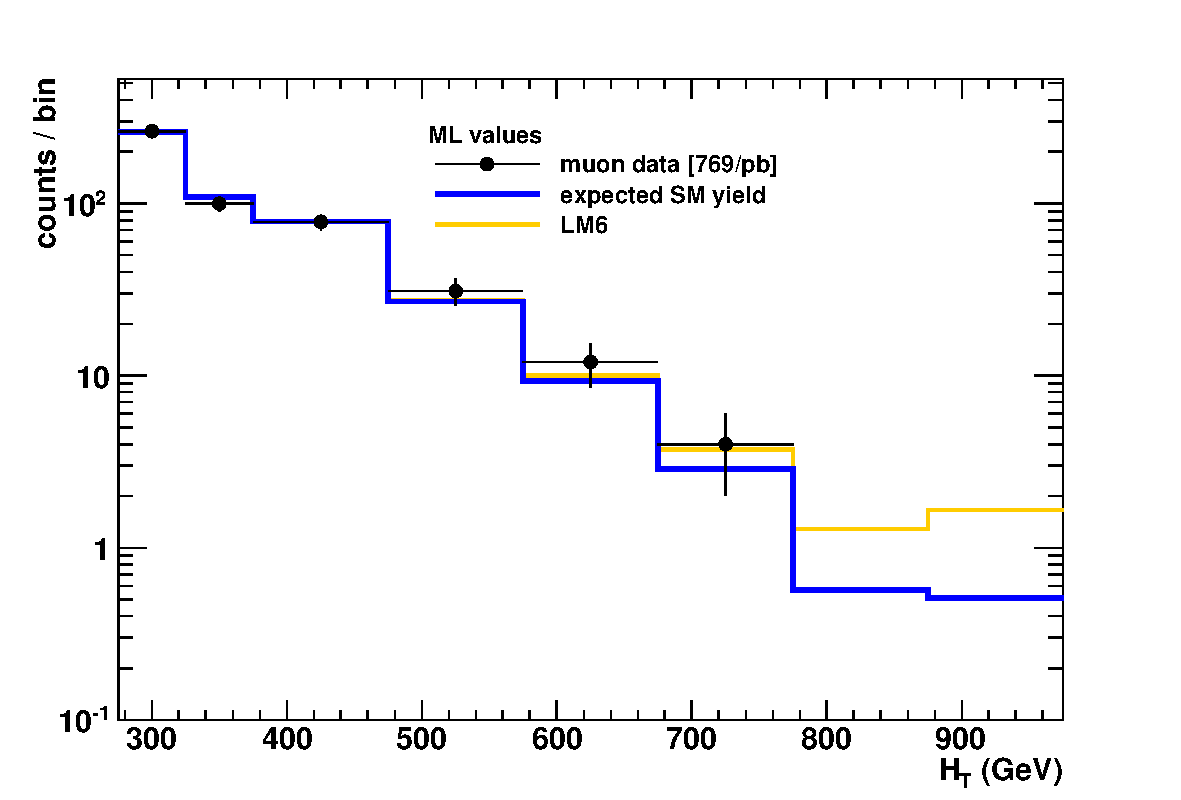
\includegraphics[width = 0.48\textwidth]{figures/stats_plots/RQcdZero/muon_control_fit_logy.pdf}
%     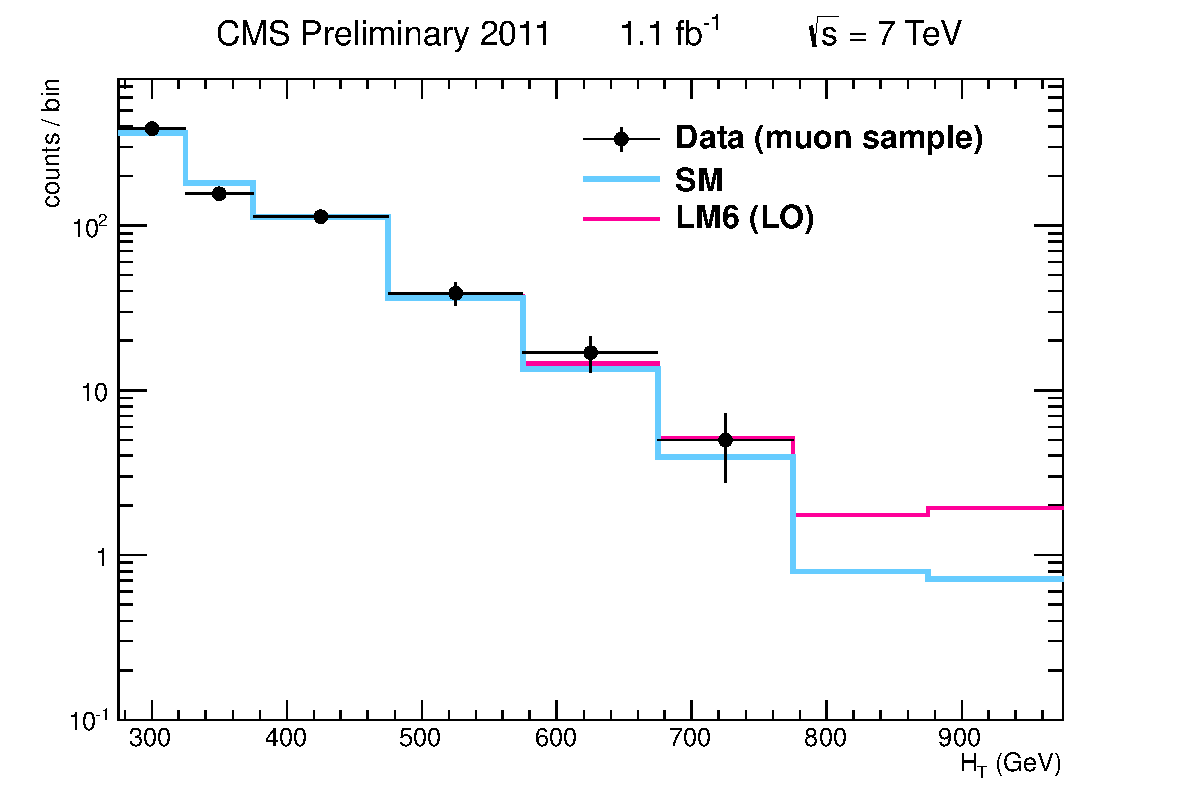
\includegraphics[width = 0.48\textwidth]{figures/stats_plots/RQcdFallingExp/muon_control_fit_logy.pdf}
%     \caption{\label{fig:muon}  \scalht distribution for events selected in the muon control sample for scenario a) (left) and scenario b) (right).
%  Shown are the events observed in data (black points), the outcome of the fit (blue line) and the MC expectation (dashed line). A possible signal
% contribution from benchmark point LM6 is indicated as well (yellow line).}
%   \end{center}
% \end{figure}

% \begin{figure}[t]
%   \begin{center}
%     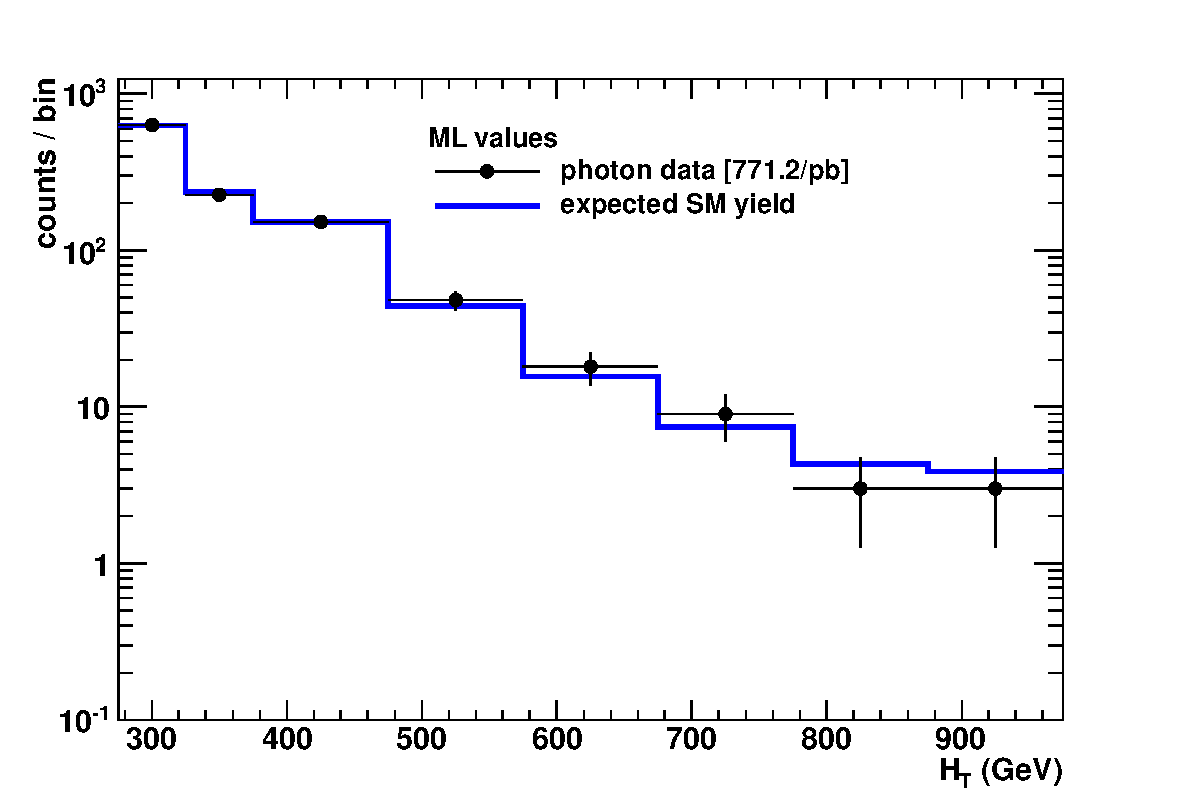
\includegraphics[width = 0.48\textwidth]{figures/stats_plots/RQcdZero/photon_control_fit_logy.pdf}
%     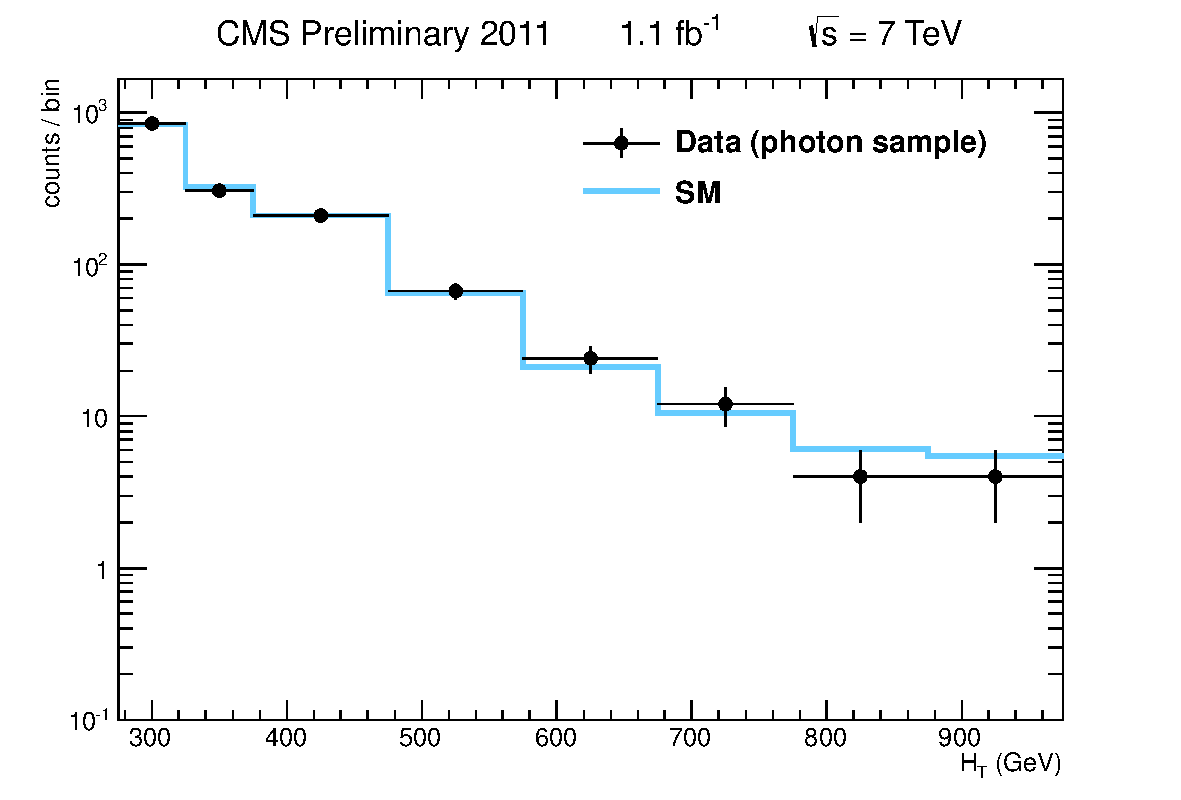
\includegraphics[width = 0.48\textwidth]{figures/stats_plots/RQcdFallingExp/photon_control_fit_logy.pdf}
%     \caption{\label{fig:photon} \scalht distribution for events selected in the photon control sample for scenario a) (left) and scenario b) (right). Shown are the events observed in data (black points), the outcome of the fit (blue line) and the MC expectation (dashed line).}
%   \end{center}
% \end{figure}

% \begin{figure}[t]
%   \begin{center}
%     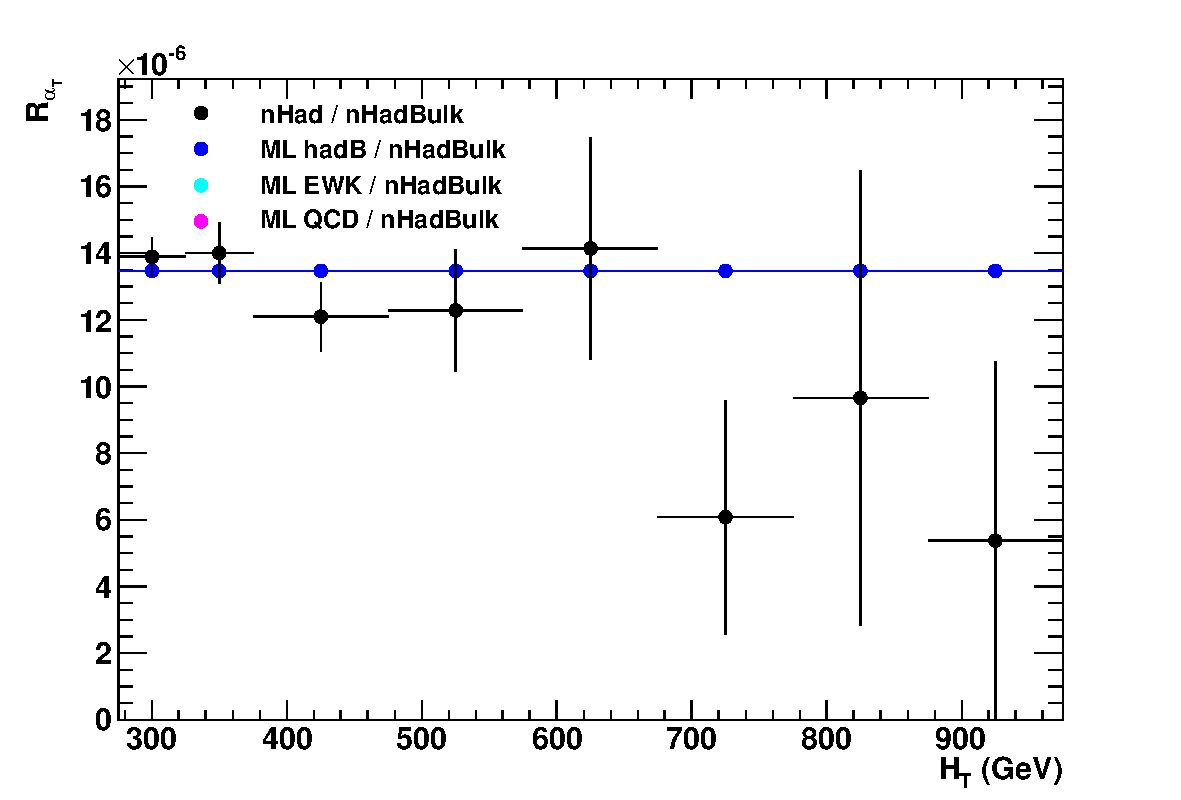
\includegraphics[width = 0.48\textwidth]{figures/stats_plots/RQcdZero/hadronic_signal_alphaT_ratio.pdf}
%     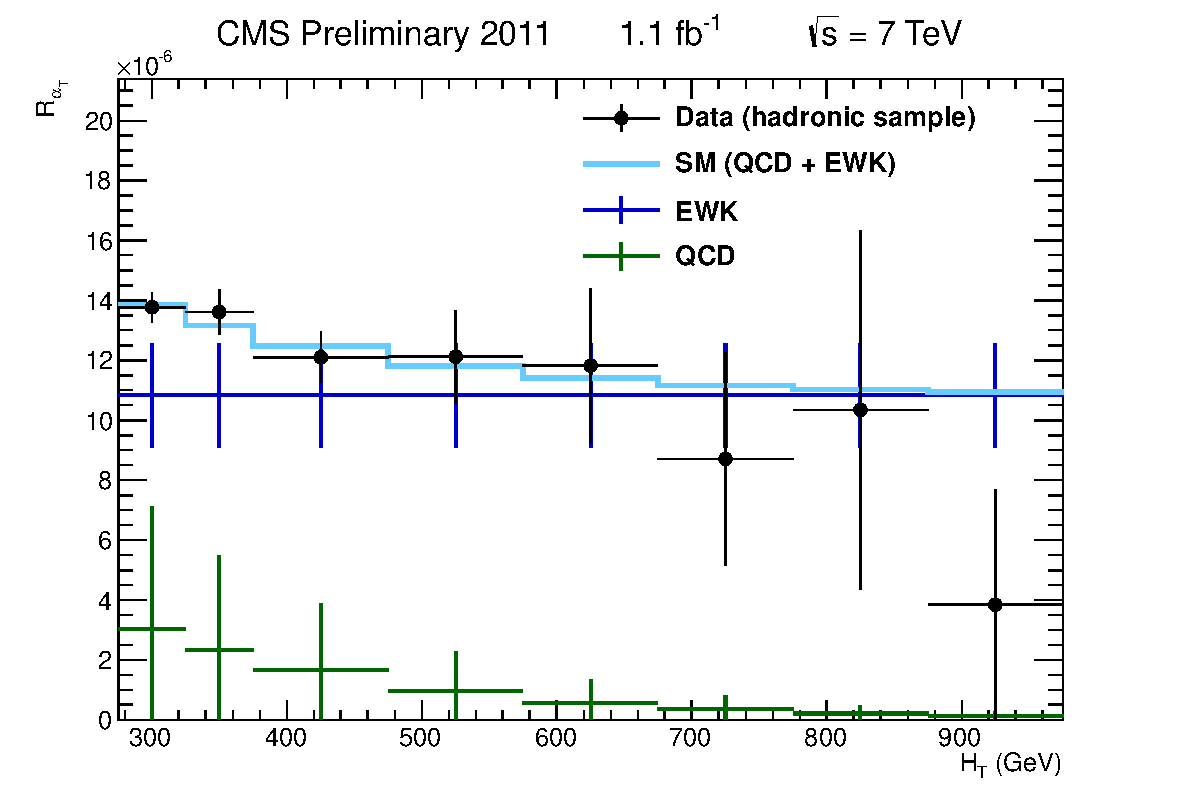
\includegraphics[width = 0.48\textwidth]{figures/stats_plots/RQcdFallingExp/hadronic_signal_alphaT_ratio.pdf}
%     \caption{\label{fig:rat} \RaT as a function of \scalht as observed in data (black points) and the results of the fit assuming different scenarios: a) (left) and b) (right) .}
%   \end{center}
% \end{figure}


\begin{figure}[t]
  \begin{center}
    \subfigure[\label{fig:hadronic} \scalht distribution for events in the hadronic signal sample. Shown are the events observed in data (black points), the outcome of the fit (light blue line) and a breakdown of the individual background contributions as predicted by the control samples. A possible signal contribution from benchmark point LM6 is indicated as well (magenta line).]{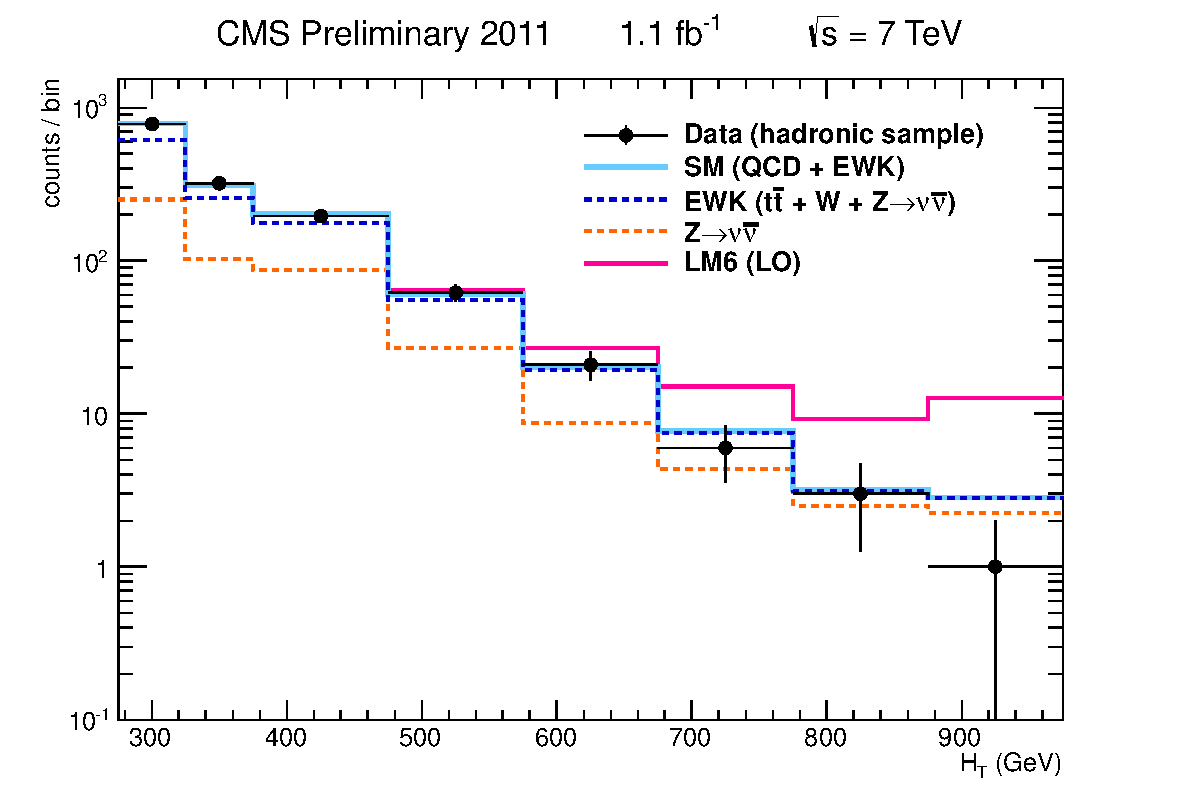
\includegraphics[width = 0.48\textwidth]{figures/stats_plots/RQcdFallingExp/hadronic_signal_fit_logy.pdf}}
\hspace{0.3cm}
    \subfigure[\label{fig:muon}  \scalht distribution for events selected in the muon control sample. Shown are the events observed in data (black points) and the outcome of the fit (light blue line). A possible signal contribution from benchmark point LM6 is indicated as well (magenta
line).]{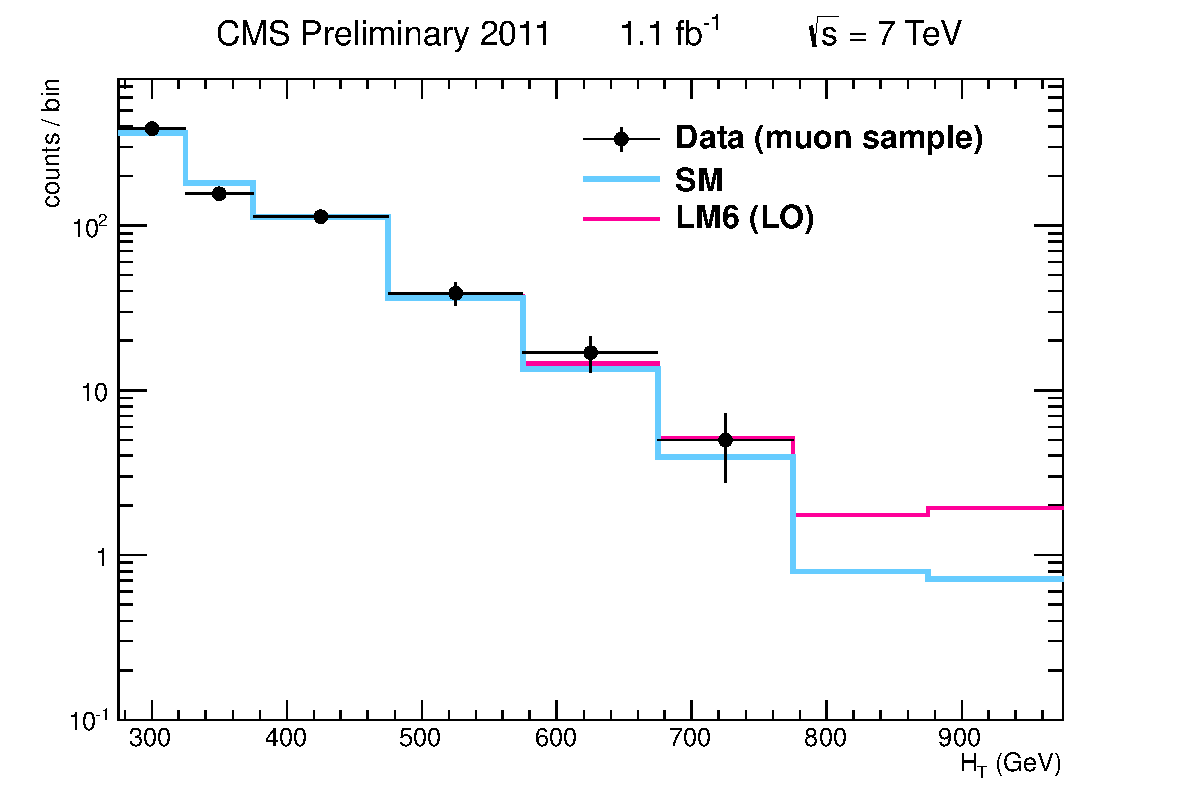
\includegraphics[width = 0.48\textwidth]{figures/stats_plots/RQcdFallingExp/muon_control_fit_logy.pdf}}\\
    \subfigure[\label{fig:photon} \scalht distribution for events
    selected in the photon control sample. Shown are the events observed in data (black points), the outcome of the fit (light blue line).]{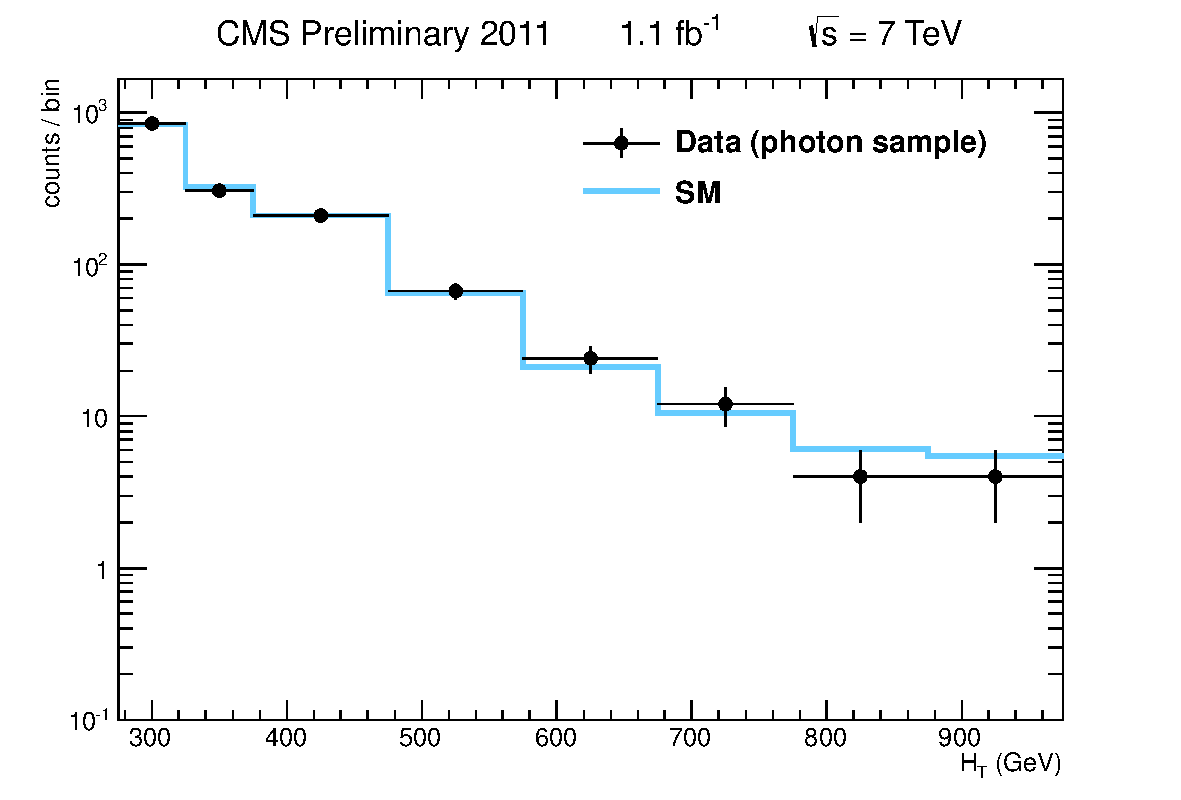
\includegraphics[width = 0.48\textwidth]{figures/stats_plots/RQcdFallingExp/photon_control_fit_logy.pdf}}
\hspace{0.3cm} 
   \subfigure[\label{fig:rat} \RaT as a function of \scalht as observed in data (black points) and the result of the fit.]{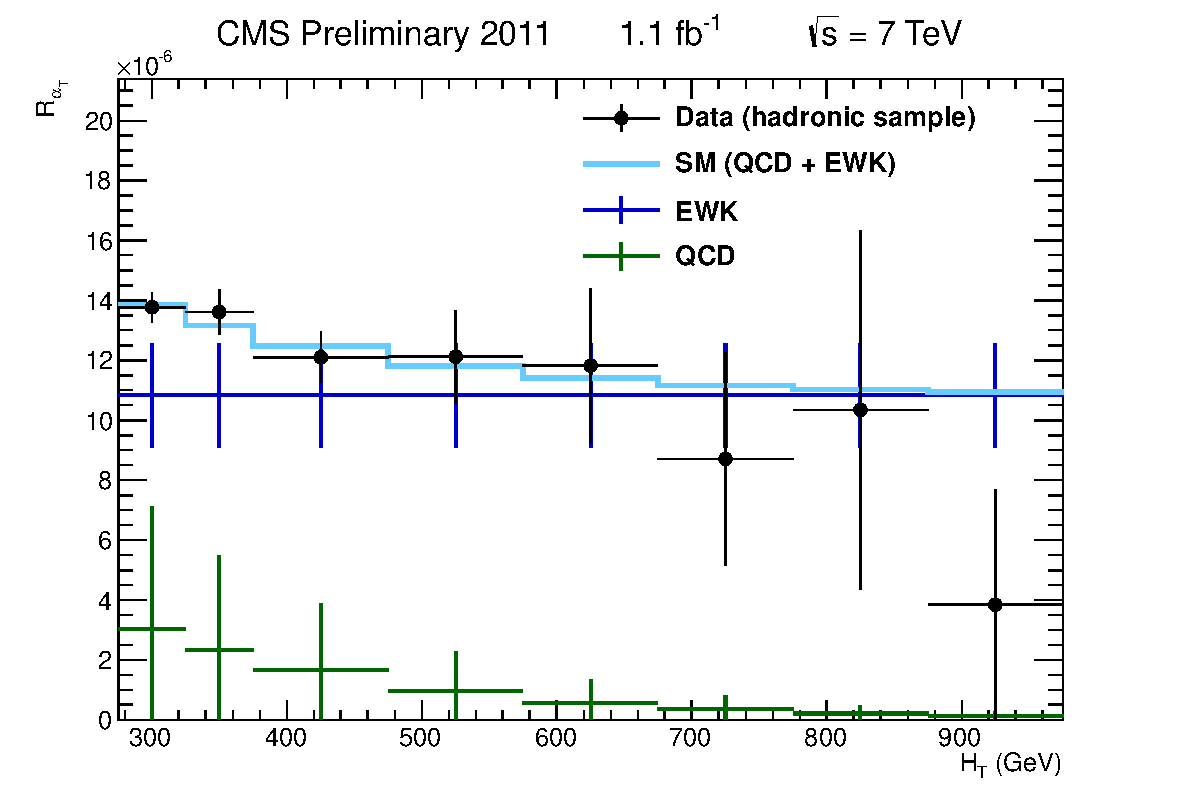
\includegraphics[width = 0.48\textwidth]{figures/stats_plots/RQcdFallingExp/hadronic_signal_alphaT_ratio.pdf}}
    \caption{\label{fig:fitresult} Result of the combined fit to the
      hadronic, muon and photon samples.
}
  \end{center}
\end{figure}





\begin{figure}[t]
  \begin{center}
    %%\includegraphics[width = 0.90\textwidth]{figures/stats_plots/RQcdFallingExp/profileLikelihood_REwkConstant_RQcdFallingExp_tanBeta10_lo_excluded95.pdf}
%    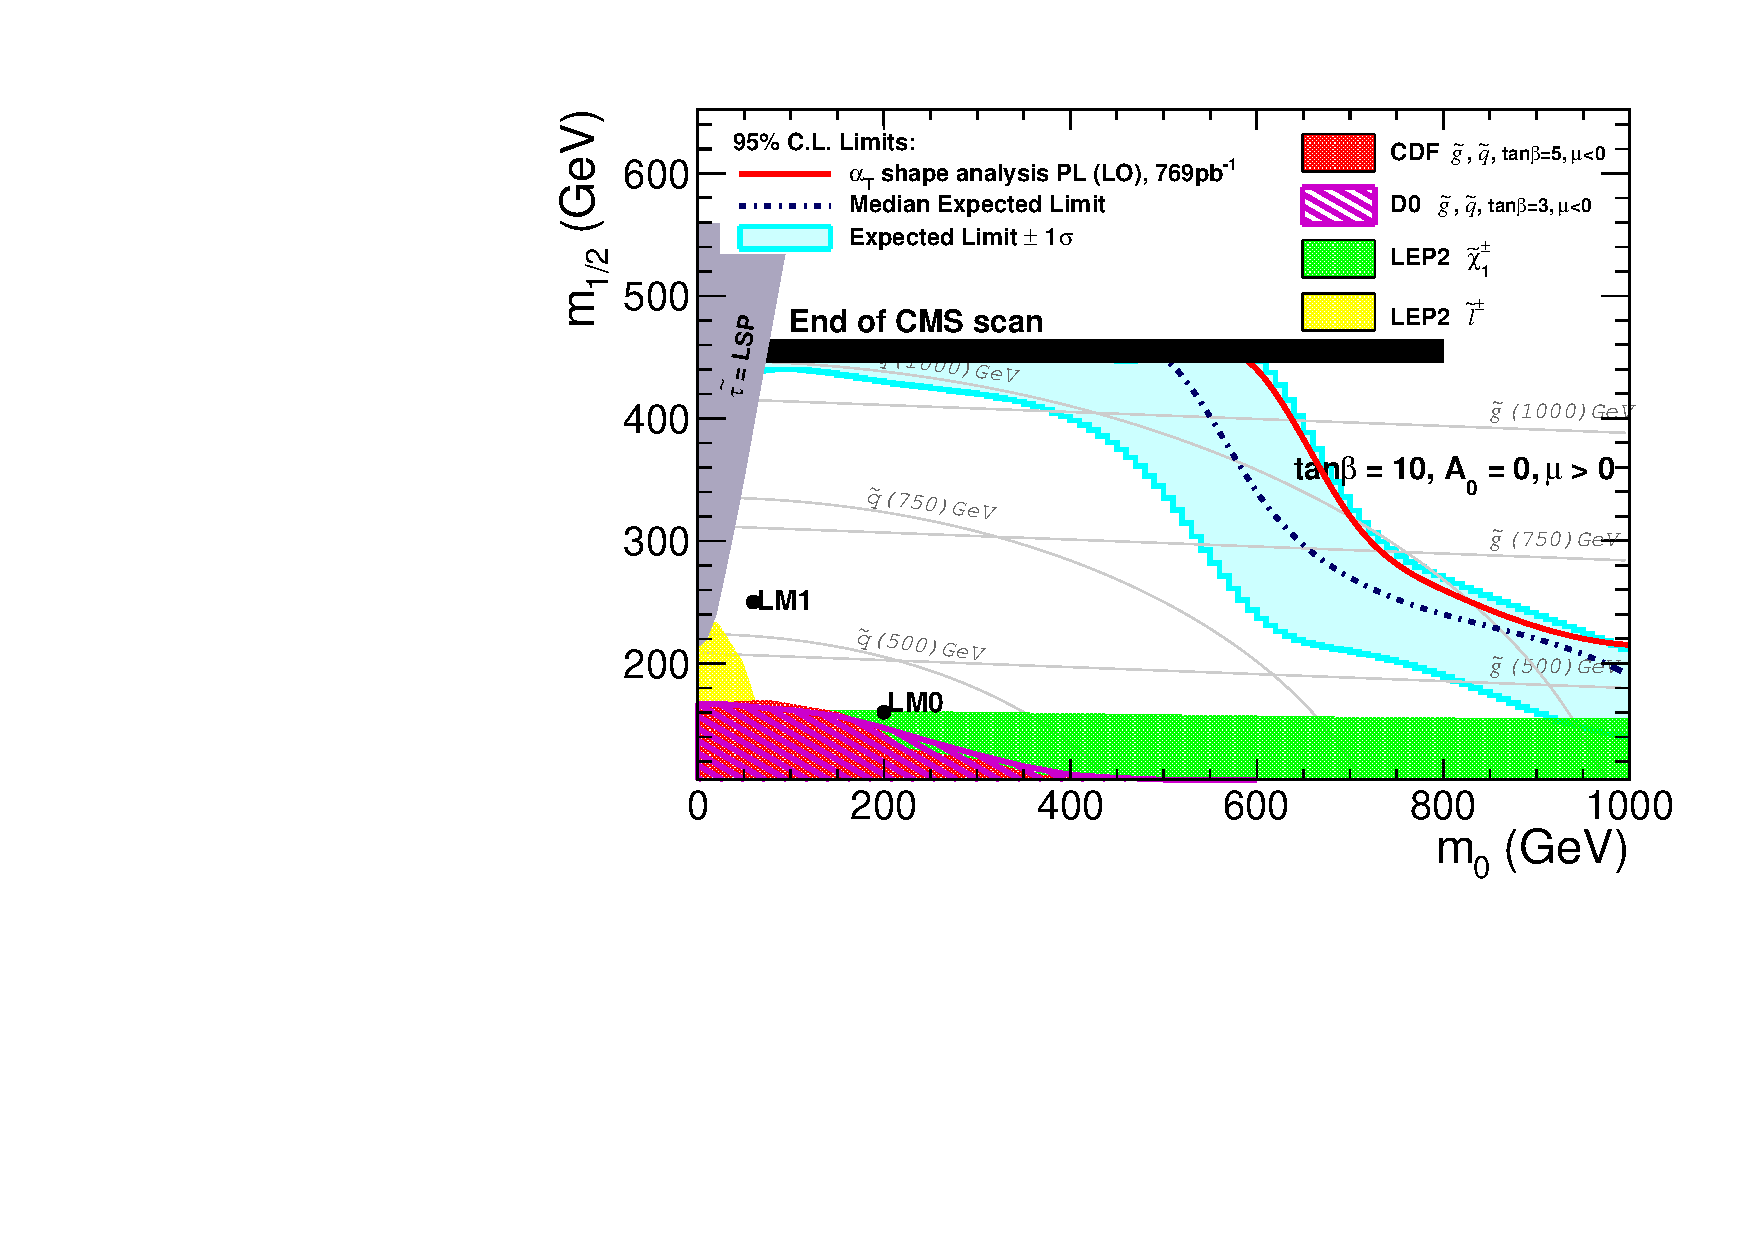
\includegraphics[width = 0.90\textwidth]{figures/RA1_ExclusionLimit_tanb10-QCDexp-770.pdf}
    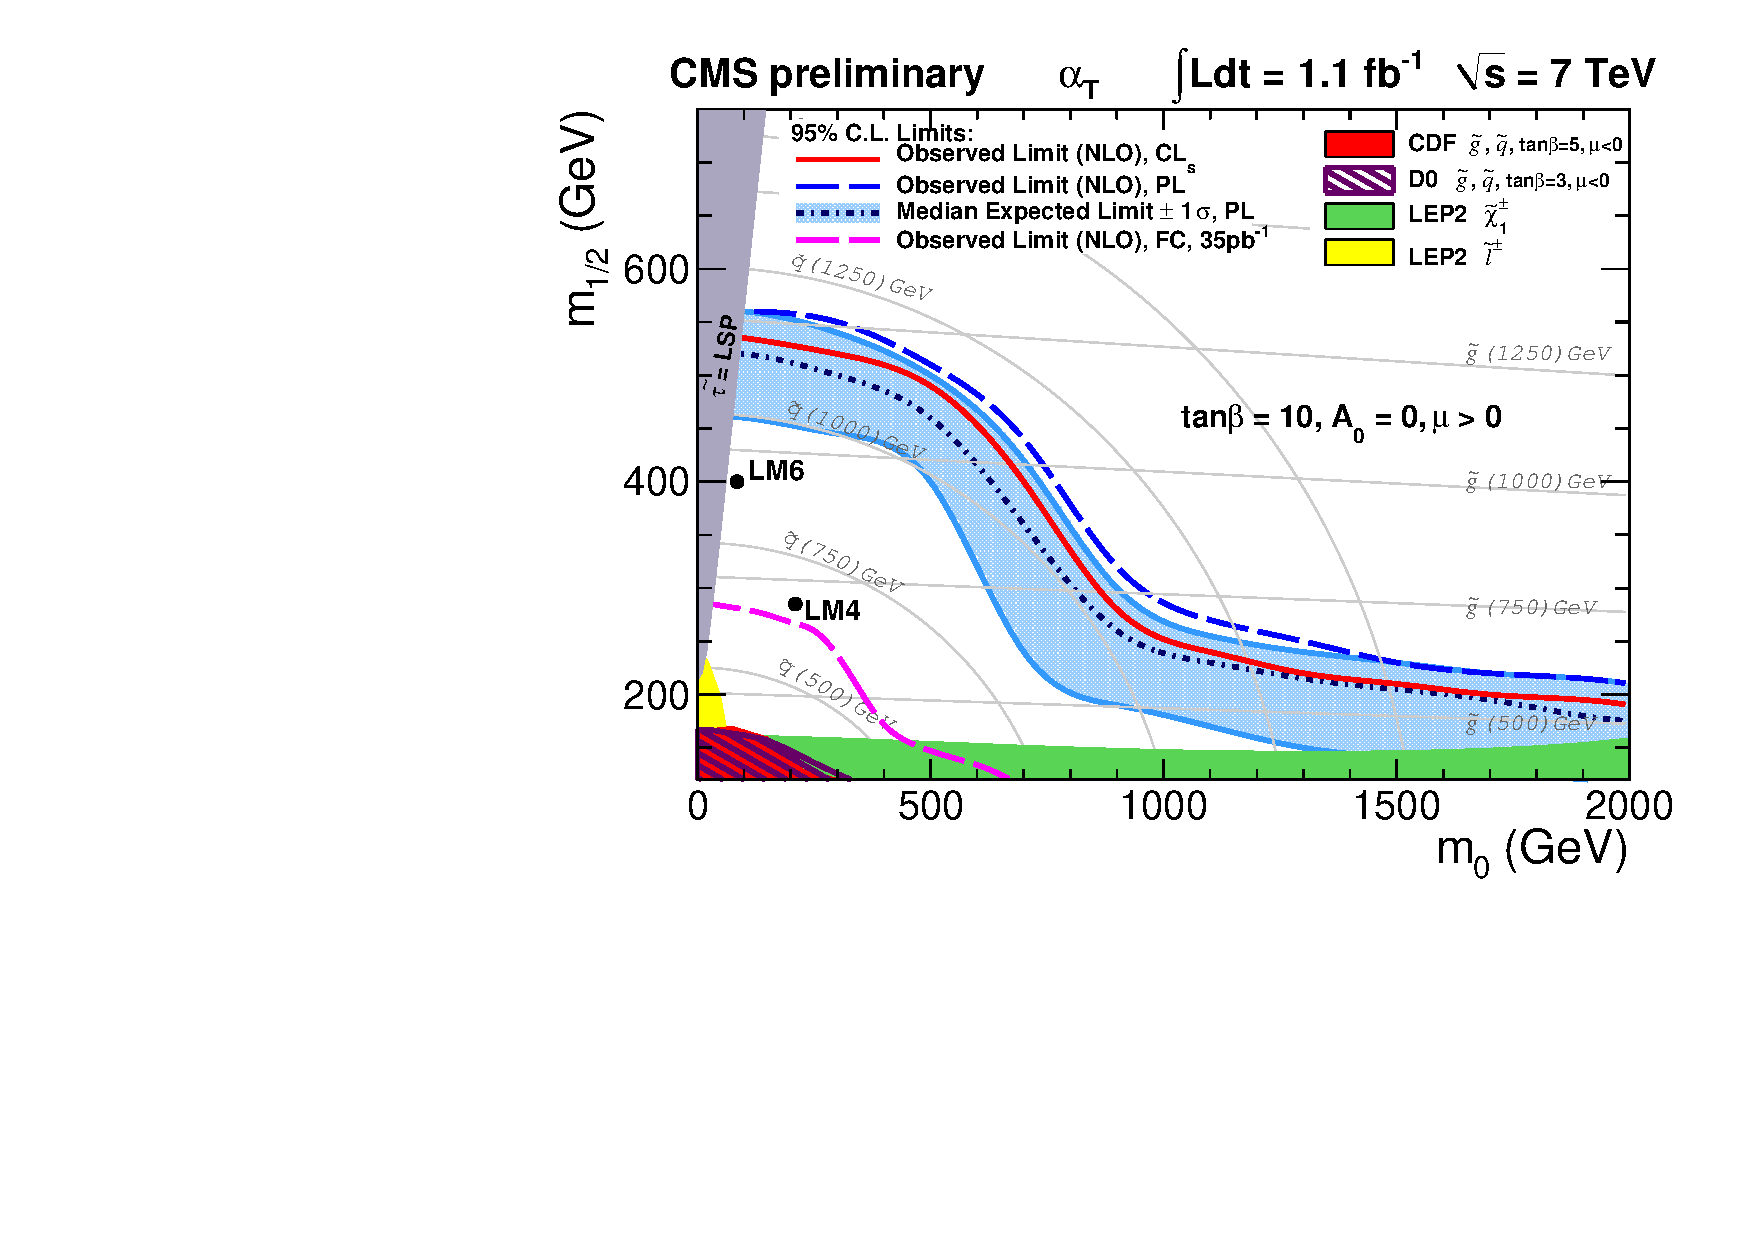
\includegraphics[width = 0.90\textwidth]{figures/RA1_ExclusionLimit_tanb10_def.pdf}
    \caption{\label{fig:cmssm} 
Observed and expected 95\% CL exclusion contours in the CMSSM ($m_0, m_{1/2}$) plane
($\tan \beta = 10, A_0 = 0, \mu > 0$) using NLO signal cross
sections using the Profile Likelihood (PL) method. The expected limit is shown with its 68\% CL range.
The observed limit using the \cls method is shown as well.
}
  \end{center}
\end{figure}



